\documentclass[a4paper, 12pt]{article}

\setlength{\textheight}{740pt} % text height 780
\setlength{\textwidth}{500pt} % text width
\setlength{\hoffset}{-20pt}
\setlength{\voffset}{-30pt}
\setlength{\topmargin}{0pt}
\setlength{\headheight}{0pt}
\setlength{\headsep}{0pt}
\setlength{\oddsidemargin}{0pt}
\setlength{\marginparsep}{0pt}
\setlength{\footskip}{40pt}

%\usepackage[T2A]{fontenc}
\usepackage[utf8]{inputenc}
\usepackage[russian]{babel}
\usepackage{multicol}
\usepackage{graphicx}
\usepackage{xcolor}
\usepackage{esvect}% vector \vv
\newcommand{\hlr}[1]{%
  \colorbox{red!50}{$\displaystyle#1$}}
\newcommand{\hly}[1]{%
  \colorbox{yellow!40}{$\displaystyle#1$}}
\newcommand{\hlt}[1]{%
  \colorbox{teal!40}{$\displaystyle#1$}}

\setlength\columnsep{113pt}
\usepackage{pgfplots}
\usepgfplotslibrary{fillbetween}
% TikZ libriries
\usepackage{tikz}
\usetikzlibrary{patterns}
\usetikzlibrary{arrows,shapes}
\usetikzlibrary{decorations.markings}
\usetikzlibrary{arrows.meta}
\usetikzlibrary{angles,quotes}
% for right angle
\usepackage{tkz-euclide}
%%%\usetkzobj{all}
% greek symbols
\usepackage[Symbol]{upgreek}
% math symbols
\usepackage{amssymb} 
\usepackage{amsmath}
%\setlength\parindent{0pt} % set noindent for entire file
\usepackage{indentfirst} % to indent the first paragraph
\linespread{1.4} % line spacing for the whole document

% create bold dash to print 
\newcommand*\bdash{\textbf{---\ }}

%\usepackage{hyperref}
\usepackage[pdfusetitle]{hyperref}
\hypersetup{colorlinks=true,urlcolor=blue,linkcolor=blue}
\title{Векторы в физике}
\author{Олег Стенякин}
\date{\today}

\begin{document}
%\thispagestyle{empty}
%%%%%%%%%%%%%%%%%%%%%%%%%%%%%%%%%%%%%%%%%%%%%%%%%%%%%%%%%%%
\part*{Векторы в физике}
%%%%%%%%%%%%%%%%%%%%%%%%%%%%%%%%%%%%%%%%%%%%%%%%%%%%%%%%%%%

\tableofcontents

\clearpage

%%%%%%%%%%%%%%%%%%%%%%%%%%%%%%%%%%%%%%%%%%%%%%%%%%%%%%%%%%%
\section{Понятие вектора}
%%%%%%%%%%%%%%%%%%%%%%%%%%%%%%%%%%%%%%%%%%%%%%%%%%%%%%%%%%%

Точки, которые являются концами произвольного отрезка, называют
\textbf{граничными точками отрезка}.

\textbf{Вектор} \bdash отрезок, для которого указано, какая из его
граничных точек считается началом, а какая \bdash концом.

Векторы обозначают двумя заглавными буквами со стрелкой над ними, например
$\vv{AB}$. Первая буква обозначает начало вектора, вторая \bdash конец.
Векторы часто обозначают одной строчной буквой со стрелкой над ней, например,
$\vv{a}$, $\vv{b}$, $\vv{c}$. В книгах векторы обозначаются жирным прямым шрифтом: 
\textbf{a}, \textbf{b}, \textbf{c}.

\begin{figure}[h]
  \centering
  \begin{tikzpicture}[thick]
    \coordinate [label=below left:$A$] (A) at (0cm,0cm);
    \coordinate [label=above:$B$](B) at (3cm,2cm);
    
    \draw [fill=black] (A) circle (1.5pt);% node [above] {A};
    \draw [fill=black] (B) circle (1.5pt);% node [right] {B};
    
    \draw [-Latex, very thick] (A) -- (B);
    
    \draw (1.2cm,1.3cm) node {$\vv{a}$};
    
    \draw (-1.9cm,0cm) node {начало вектора};
    \draw (4.8cm,2.0cm) node {конец вектора};
  \end{tikzpicture}
  \caption{\small Вектор.}\label{pic:vec}
\end{figure}

Любая точка плоскости также является вектором. В этом случае вектор называется
\textbf{нулевым}. Начало нулевого вектора совпадает с его концом, на рисунке
такой вектор изображается точкой. Обозначается нулевой вектор так: $\vv{MM}$ или $\vv{0}$.

\textbf{Длиной} или \textbf{модулем} ненулевого \textbf{вектора} $\vv{AB}$ называется длина отрезка $AB$.
Длина вектора обозначается так: $|\vv{AB}|$, $|\vv{a}|$ или просто буквой без стрелки $a$.
Длина нулевого вектора равна нулю: $|\vv{0}| = 0$.

В физике в отличие от геометрии модули величин имеют \textbf{размерность}.
Например, модуль скорости измеряется
в метрах в секунду (м/с), модуль силы \bdash в ньютонах (Н), модуль напряжённости электрического
поля \bdash в вольтах на метр (В/м), модуль индукции магнитного поля \bdash в теслах (Тл) и т.д.
 % Понятие вектора

\clearpage

%%%%%%%%%%%%%%%%%%%%%%%%%%%%%%%%%%%%%%%%%%%%%%%%%%%%%%%%%%%
\section{Равенство векторов}
%%%%%%%%%%%%%%%%%%%%%%%%%%%%%%%%%%%%%%%%%%%%%%%%%%%%%%%%%%%
Ненулевые векторы называются \textbf{коллинеарными}, если они лежат или на одной прямой,
или на параллельных прямых. Нулевой вектор считается коллинеарным любому вектору.

На рисунке векторы $\vv{a}$, $\vv{b}$, $\vv{c}$ и $\vv{d}$ коллинеарны, а
вектор $\vv{e}$ не коллинеарен ни одному из векторов.

Если два ненулевых вектора коллинеарны, то они могут быть направлены или одинаково,
или противоположно. В первом случае векторы называются \textbf{сонаправленными}, а во втором
\bdash \textbf{противоположно направленными}.

На рисунке~\ref{pic:vec_coll} векторы $\vv{a}$ и $\vv{b}$
сонаправлены ($\vv{a}\uparrow\uparrow\vv{b}$),
а векторы $\vv{c}$ и $\vv{d}$ противоположно направлены ($\vv{c}\uparrow\downarrow\vv{d}$).

Векторы называются \textbf{противоположными}, если они противоположно направлены и их длины равны.
Вектор, противоположный вектору $\vv{a}$ обозначается $-\vv{a}$.

Векторы называются \textbf{равными}, если они сонаправлены и их длины равны.

Таким образом, векторы $\vv{a}$ и $\vv{b}$ равны, если $\vv{a}\uparrow\uparrow\vv{b}$
и $|\vv{a}|=|\vv{b}|$. Равенство векторов обозначается так: $\vv{a}=\vv{b}$.

\begin{figure}[h]
  \centering
  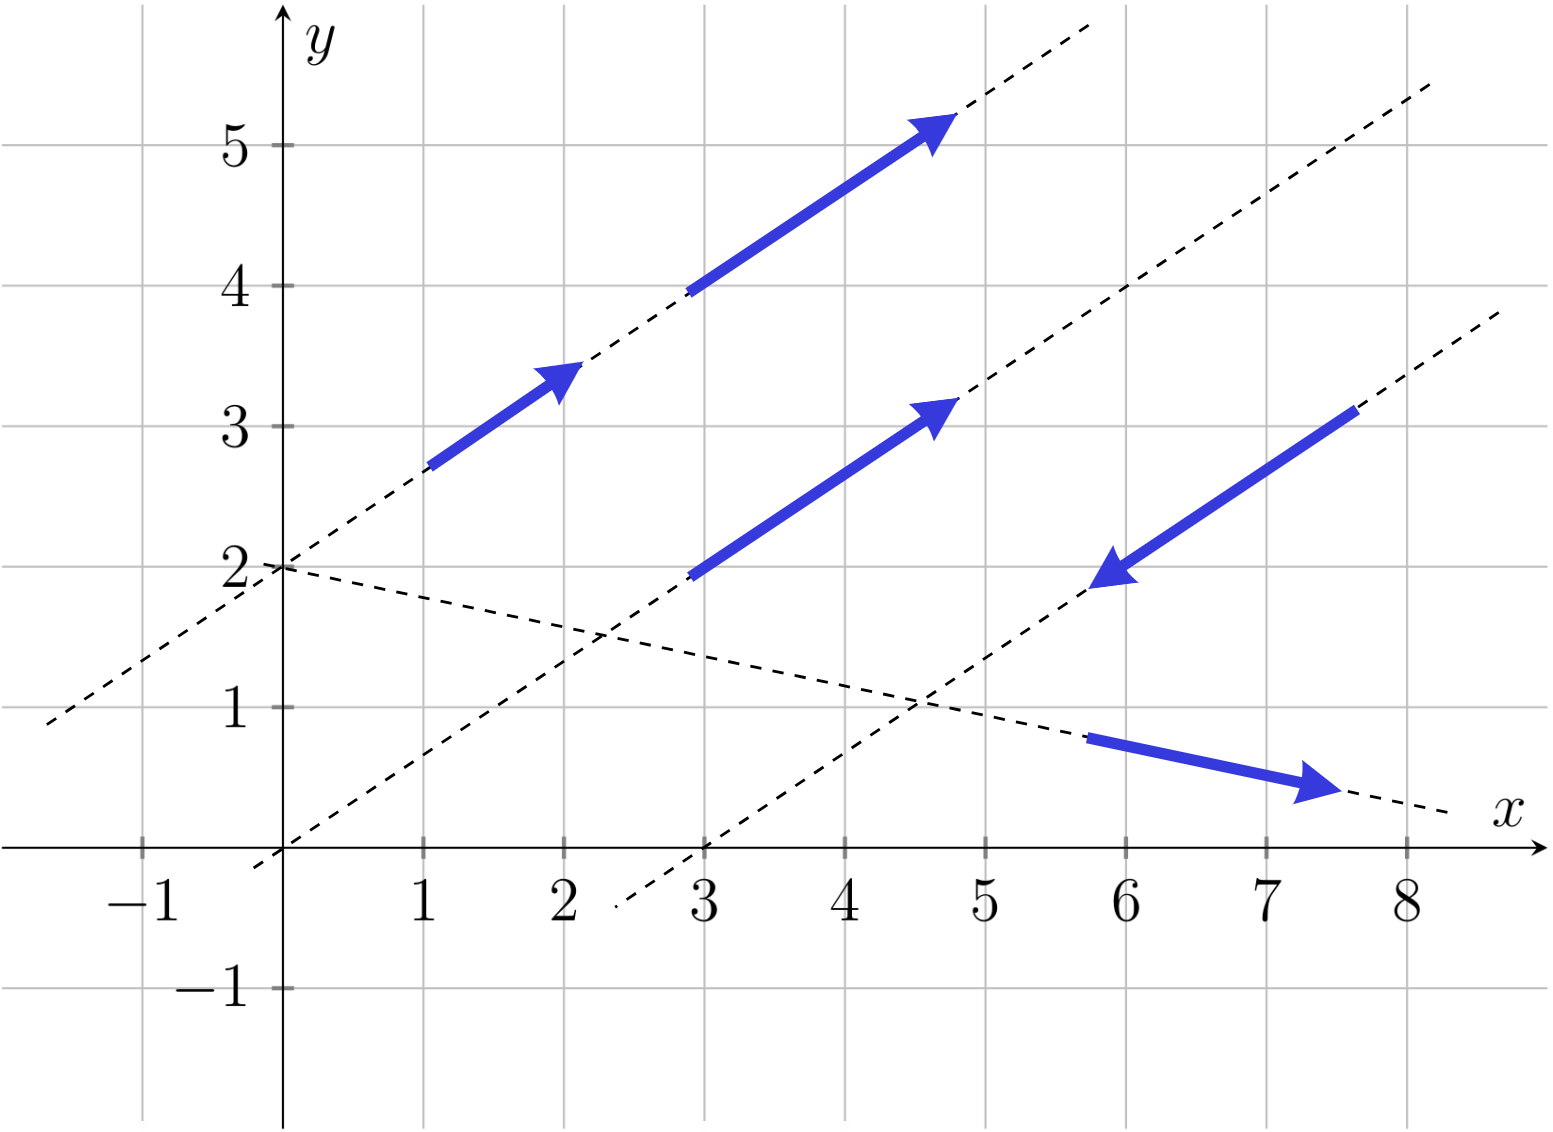
\includegraphics[width=0.7\textwidth]{pics/axis_l.png}
  \put(-180,215){\large $\vv{a}$}
  \put(-250,170){\large $\vv{c}$}
  \put(-180,150){\large $\vv{b}$}
  \put(-90,150){\large $\vv{d}$}
  \put(-80,90){\large $\vv{e}$}
  \caption{\small Коллинеарные и неколлинеарные векторы.}\label{pic:vec_coll}
\end{figure}

\clearpage

Если точка $A$ \bdash начало вектора $\vv{a}$, то говорят, что вектор $\vv{a}$
\textbf{отложен от точки} $A$. Верно следующее утверждение: от любой точки $M$ можно отложить
вектор, равный данному, и при том только один.

Равные векторы, отложенные от разных точек, часто обозначают одной и той же буквой.
Иногда говорят, что это один и тот же вектор, отложенный от разных точек.

%\begin{center}
%  \begin{tikzpicture}
%    \begin{axis}[
%        axis lines=middle,
%        axis equal image,
%        grid=major,
%        xmin=-2,
%        xmax=9,
%        ymin=-2,
%        ymax=6,
%        xlabel=$x$,
%        ylabel=$y$,
%        xtick={-1,...,8},
 %       ytick={-1,...,5},
%        tick style={thick},
%        width=12cm
%      ]
%    \end{axis}
%    \coordinate (A) at (3cm,5cm);
%    \coordinate (B) at (6cm,8cm);
%    %\draw [-latex, thick] (A) -- (B);
%    %\draw (1.2cm,1.3cm) node {$\vv{a}$};
%    \coordinate (C) at (0cm,0cm);
%    \coordinate (D) at (3cm,2cm);
%    \coordinate (E) at (0cm,0cm);
 %   \coordinate (F) at (3cm,2cm);
%    \coordinate (G) at (0cm,0cm);
%    \coordinate (H) at (3cm,2cm);
%    
%  \end{tikzpicture}
%\end{center}

Рисунок~\ref{pic:auto} иллюстрирует направление скоростей автомобилей,
когда их скорости сонаправлены, противоположно направлены, равны и противоположны.

\begin{figure}[h]
  \centering
  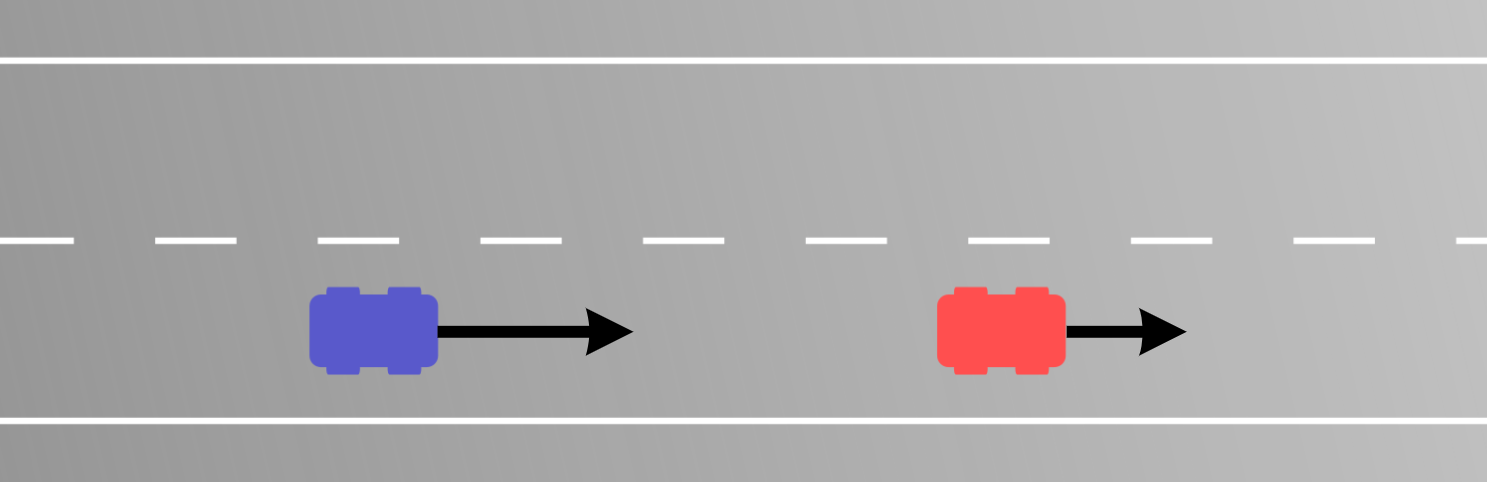
\includegraphics[width=0.48\textwidth]{pics/auto1.png}
  \put(-155,33){\large $\vv{v_1}$}
  \put(-65,33){\large $\vv{v_2}$}
  \put(-200,88){скорости сонаправлены $\vv{v_1}\uparrow\uparrow\vv{v_2}$}\hspace*{7mm}
  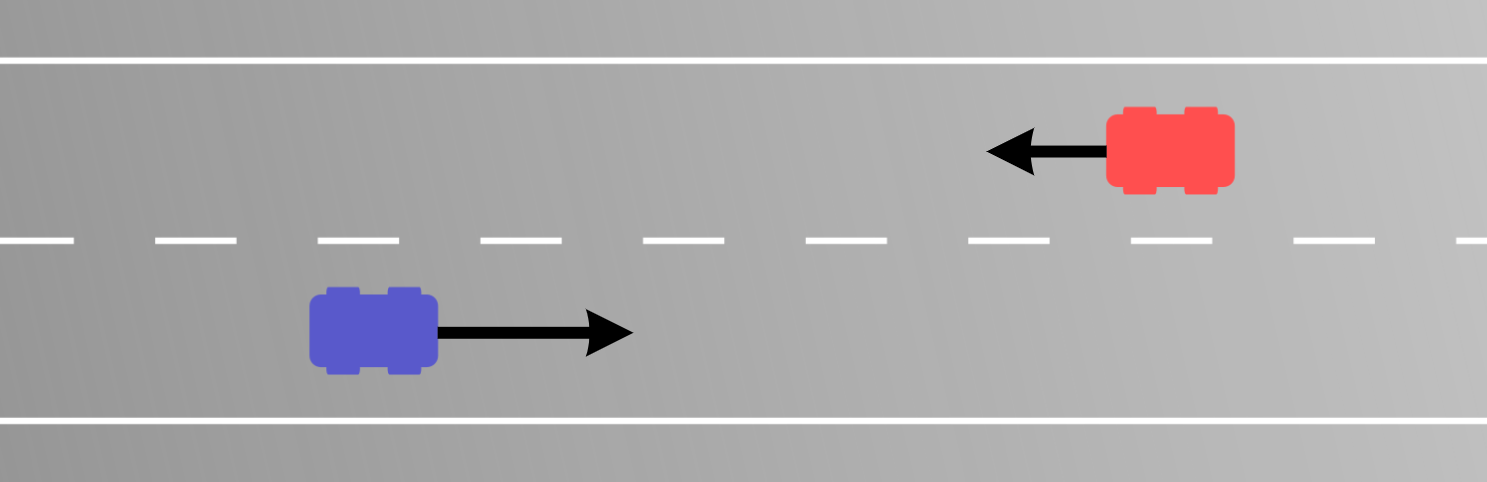
\includegraphics[width=0.48\textwidth]{pics/auto4.png}
  \put(-155,33){\large $\vv{v_1}$}
  \put(-75,65){\large $\vv{v_2}$}
  \put(-245,88){скорости противоположно направлены $\vv{v_1}\uparrow\downarrow\vv{v_2}$}
  \vspace{5mm}
  
  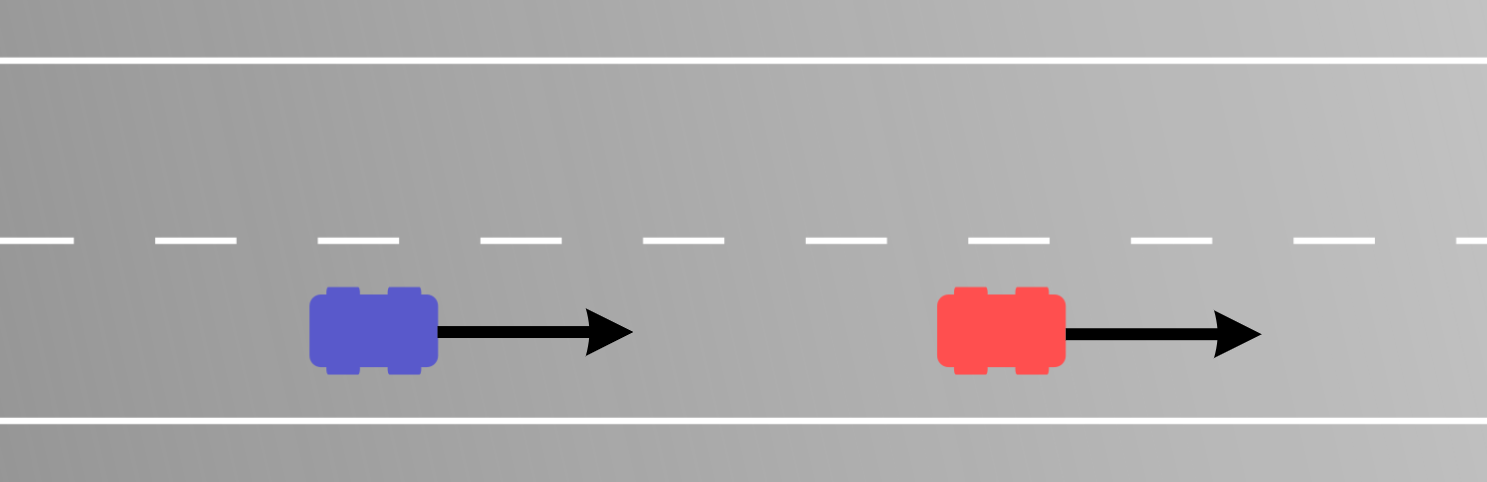
\includegraphics[width=0.48\textwidth]{pics/auto2.png}
  \put(-155,33){\large $\vv{v_1}$}
  \put(-55,33){\large $\vv{v_2}$}
  \put(-190,88){скорости равны $\vv{v_1}=\vv{v_2}$}\hspace*{7mm}
  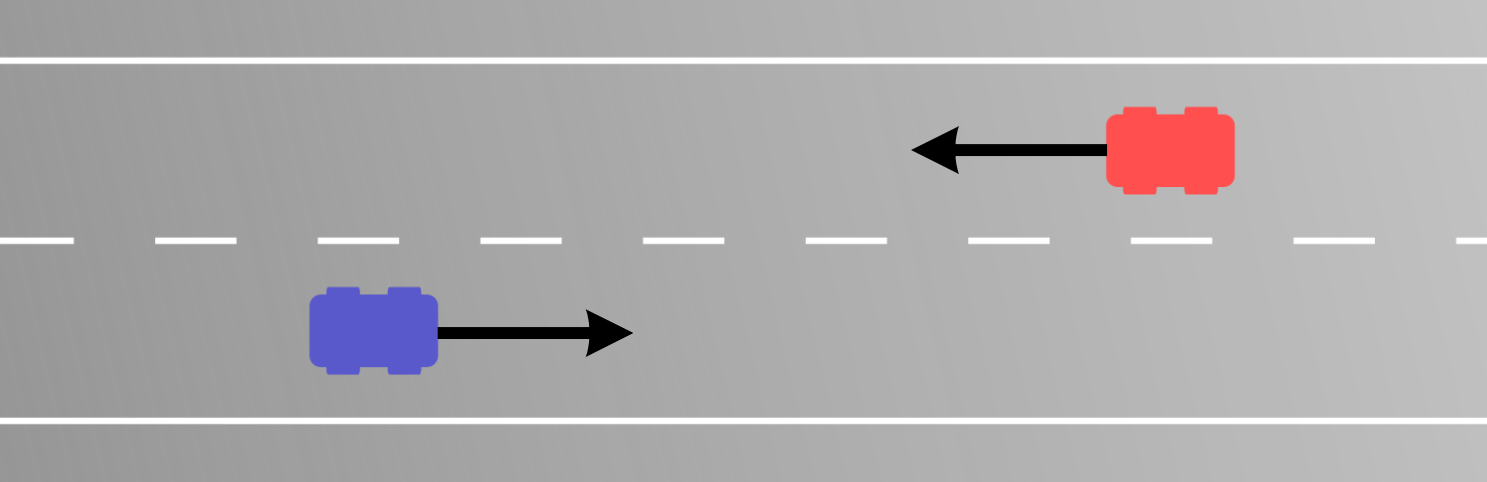
\includegraphics[width=0.48\textwidth]{pics/auto3.png}
  \put(-155,33){\large $\vv{v_1}$}
  \put(-85,65){\large $\vv{v_2}$}
  \put(-220,88){скорости противоположны $\vv{v_1}=-\vv{v_2}$}
  \caption{\small Сонаправленные, противоположно направленные, равные и
  противоположные скорости автомобилей.}\label{pic:auto}
\end{figure}
 % Равенство векторов

\clearpage

%%%%%%%%%%%%%%%%%%%%%%%%%%%%%%%%%%%%%%%%%%%%%%%%%%%%%%%%%%%
\section{Умножение вектора на число}
%%%%%%%%%%%%%%%%%%%%%%%%%%%%%%%%%%%%%%%%%%%%%%%%%%%%%%%%%%%
\textbf{Произведением} ненулевого вектора $\vv{a}$ на число $k$
называется такой вектор $\vv{b}$,
длина которого равна $|k|\cdot|\vv{a}|$, причём векторы $\vv{a}$ и $\vv{b}$
сонаправлены при $k\geqslant 0$
и противоположно направлены при $k<0$.

Произведением нулевого вектора на любое число считается нулевой вектор.

\begin{figure}[h]
  \centering
  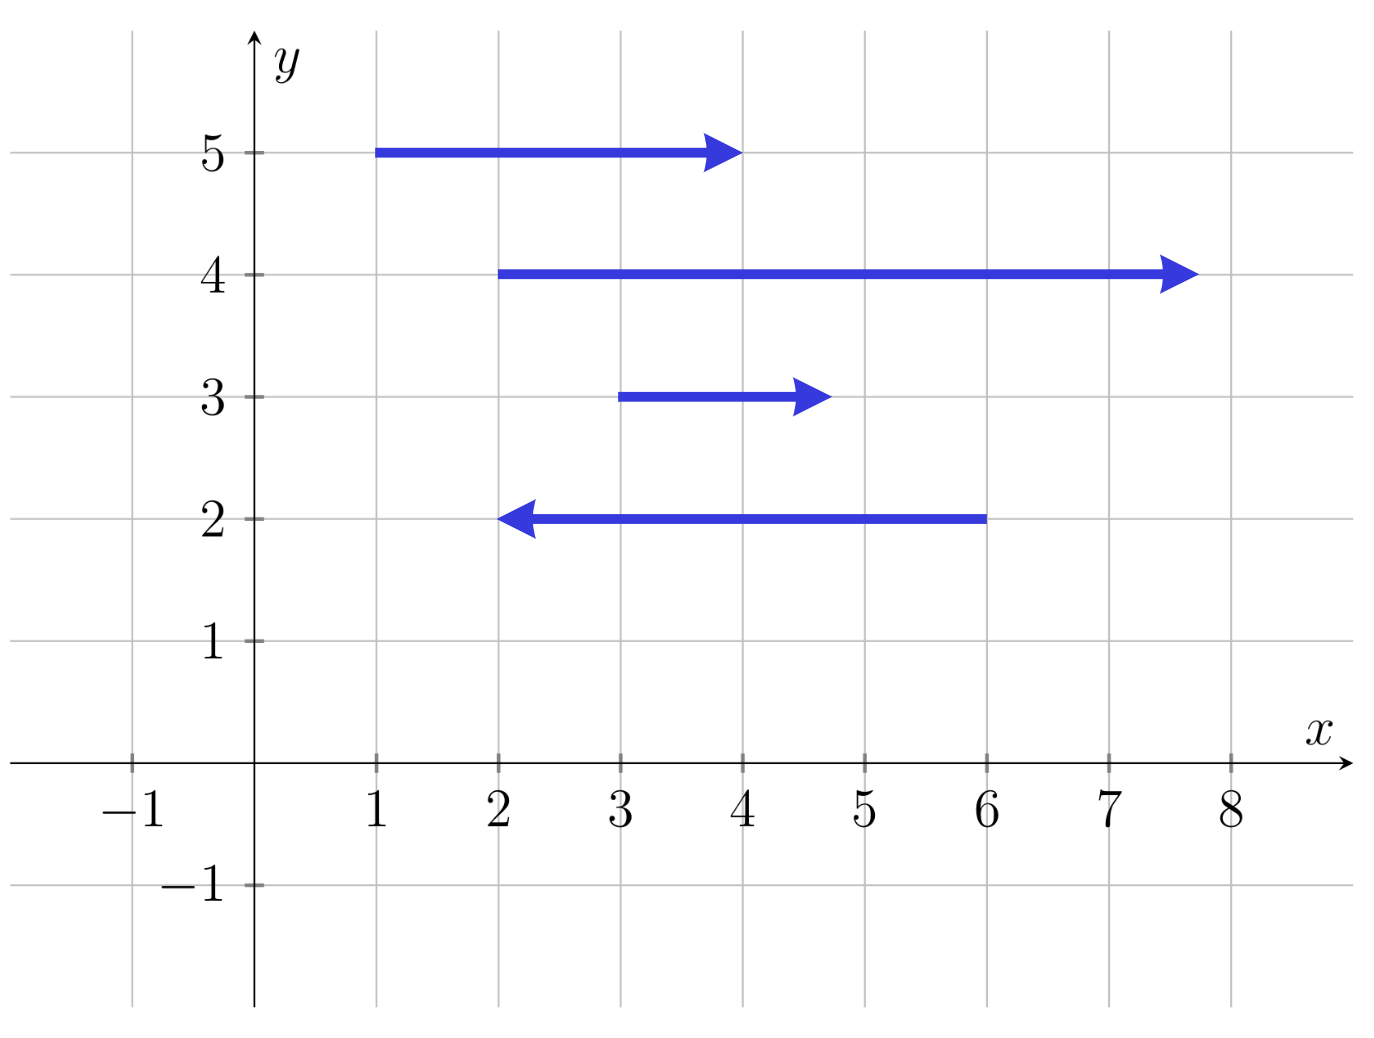
\includegraphics[width=0.7\textwidth]{pics/axis_times.png}
  \put(-210,235){$\vv{a}$}
  \put(-150,202){$\vv{b}$}
  \put(-175,170){$\vv{c}$}
  \put(-185,140){$\vv{d}$}
  \caption{\small Умножение вектора на число.}\label{pic:times}
\end{figure}

На рисунке~\ref{pic:times} изображён вектор $\vv{a}$ и векторы:
\begin{itemize}
\item $\vv{b} = k\cdot \vv{a}$, где $k>1$. В таком случае вектор $\vv{a}$
удлиняется и сохраняет прежнее направление,
\item $\vv{c} = l\cdot \vv{a}$, где $1>l>0$. В этом случае вектор $\vv{a}$ 
укорачивается и также сохраняет прежнее направление,
\item $\vv{d} = m\cdot \vv{a}$, где $m<0$. Вектор $\vv{a}$
меняет направление на противоположное.
\end{itemize}

\clearpage

Приведём \textbf{конкретные примеры}. На рисунке~\ref{pic:times_ex} изображён
вектор $\vv{a}$ длиной 2 клетки (2 единицы измерения отрезков).
А также изображены векторы:
\begin{itemize}
\item $\vv{b} = 2\vv{a}$ (удлинённый в 2 раза вектор $\vv{a}$),
\item $\vv{c} = 1/2\vv{a}$ (укороченный в 2 раза вектор $\vv{a}$),
\item $\vv{d} = -1/2\vv{a}$ (укороченный в 2 раза вектор $\vv{a}$
  и противоположно направленный),
\item $\vv{e} = -\vv{a}$ (равный по модулю вектору $\vv{a}$
  и противоположно направленный),
\item $\vv{f} = -3\vv{a}$ (удлинённый в 3 раза вектор $\vv{a}$
  и противоположно направленный).
\end{itemize}

\begin{figure}[ht]
  \centering
  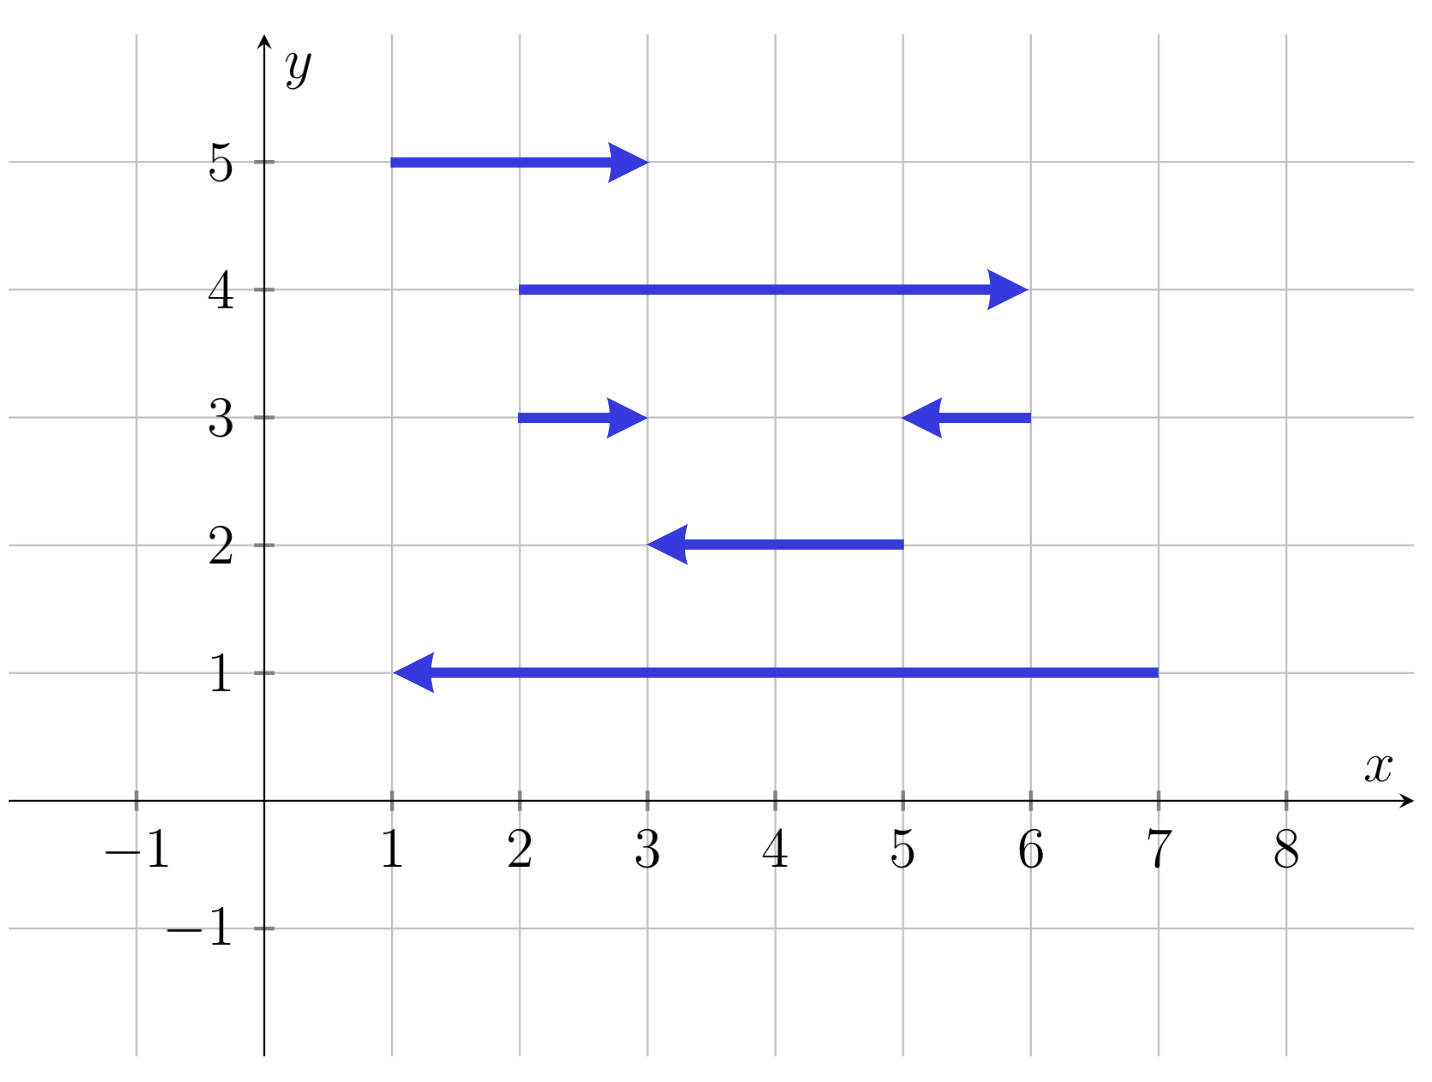
\includegraphics[width=0.7\textwidth]{pics/axis_times_ex.png}
  \put(-230,233){$\vv{a}$}
  \put(-180,203){$\vv{b} = 2\vv{a}$}
  \put(-240,170){$\vv{c} = 1/2\vv{a}$}
  \put(-140,170){$\vv{d} = -1/2\vv{a}$}
  \put(-180,140){$\vv{e} = -\vv{a}$}
  \put(-220,110){$\vv{f} = -3\vv{a}$}
  \caption{\small Умножение вектора на число, примеры.}\label{pic:times_ex}
\end{figure}


 % Умножение вектора на число

\clearpage

%%%%%%%%%%%%%%%%%%%%%%%%%%%%%%%%%%%%%%%%%%%%%%%%%%%%%%%%%%%
\section{Сложение векторов}
%%%%%%%%%%%%%%%%%%%%%%%%%%%%%%%%%%%%%%%%%%%%%%%%%%%%%%%%%%%
\subsection{Правило треугольника}
%%%%%%%%%%%%%%%%%%%%%%%%%%%%%%%%%%%%%%%%%%%%%%%%%%%%%%%%%%%
Пусть $\vv{a}$ и $\vv{b}$ \bdash два вектора. Отметим произвольную точку $A$
и отложим от этой точки вектор $\vv{AB}$, равный $\vv{a}$. Затем от точки $B$
(конец вектора $\vv{AB}$) отложим вектор $\vv{BC}$, равный $\vv{b}$.
Вектор $\vv{AC}=\vv{c}$ называется \textbf{суммой векторов} $\vv{a}$ и $\vv{b}$.

Таким образом, при построении суммы двух векторов начало второго вектора
примыкает с концу первого и сумма замыкает образуемый ими треугольник.
\begin{figure}[h]
  \centering
  \begin{tikzpicture}[thick]
    \coordinate [label=below left:$A$] (A) at (0cm,0cm);
    \coordinate [label=above:$B$] (B) at (3cm,3cm);
    \coordinate [label=above:$C$](C) at (7cm,3cm);
    \coordinate (D) at (-6cm,0cm);
    \coordinate (E) at (-3cm,3cm);
    \coordinate (F) at (-5cm,4cm);
    \coordinate (G) at (-1cm,4cm);
    
    \draw [blue, -Latex, very thick] (A) -- node[above left,black] {\large $\vv{a}$} (B);
    \draw [blue, -Latex, very thick] (B) -- node[above,black] {\large $\vv{b}$} (C);
    \draw [red, -Latex, very thick] (A) -- node[below right,black] {\large $\vv{c} =\vv{a}+\vv{b}$} (C);
    \draw [blue, -Latex, very thick] (D) -- node[above left,black] {\large $\vv{a}$} (E);
    \draw [blue, -Latex, very thick] (F) -- node[above,black] {\large $\vv{b}$} (G);
    
    \draw [fill=black] (A) circle (1.5pt);% node [above] {A};
    \draw [fill=black] (B) circle (1.5pt);% node [right] {B};
    \draw [fill=black] (C) circle (1.5pt);
  \end{tikzpicture}
  \caption{\small Сложение векторов по правилу треугольника.}\label{pic:sum_tr}
\end{figure}

По правилу треугольника \textbf{удобно складывать}
последовательные или одновременные
\textbf{перемещения}.
\begin{figure}[h]
  \centering
  \begin{tikzpicture}[thick]
    \coordinate (A) at (0cm,0cm);
    \coordinate (B) at (3cm,3cm);
    \coordinate (C) at (7cm,3cm);

    \draw [blue, -Latex, very thick] (A) -- node[above left,black] {\large $\vv{s_1}$} (B);
    \draw [blue, -Latex, very thick] (B) -- node[above,black] {\large $\vv{s_2}$} (C);
    \draw [red, -Latex, very thick] (A) -- node[below right,black] {\large $\vv{s} =\vv{s_1}+\vv{s_2}$} (C);
  \end{tikzpicture}
  \caption{\small Сложение перемещений по правилу треугольника.}\label{pic:sum_perem}
\end{figure}

\clearpage

%%%%%%%%%%%%%%%%%%%%%%%%%%%%%%%%%%%%%%%%%%%%%%%%%%%%%%%%%%%
\subsection{Правило параллелограмма}
%%%%%%%%%%%%%%%%%%%%%%%%%%%%%%%%%%%%%%%%%%%%%%%%%%%%%%%%%%%
Для построения суммы двух векторов $\vv{a}$ и $\vv{b}$
по правилу параллелограмма отметим произвольную точку $A$
и отложим от этой точки вектор $\vv{AB}$, равный $\vv{a}$.
Затем от этой же точки отложим вектор $\vv{AD}$, равный $\vv{b}$.
Вектор $\vv{AC}=\vv{c}$ называется \textbf{суммой векторов} $\vv{a}$ и $\vv{b}$.

Таким образом, при построении суммы двух векторов $\vv{a}$ и $\vv{b}$
начала векторов совмещаются,
и на них как на сторонах строится параллелограмм. Диагональ этого параллелограмма,
проведённая из общего начала складываемых векторов, называется их суммой.

\begin{figure}[h]
  \centering
  \begin{tikzpicture}[thick]
    \coordinate [label=below left:$A$](A) at (0cm,0cm);
    \coordinate [label=above:$B$](B) at (3cm,3cm);
    \coordinate [label=above:$C$](C) at (7cm,3cm);
    \coordinate (D) at (-6cm,0cm);
    \coordinate (E) at (-3cm,3cm);
    \coordinate (F) at (-5cm,4cm);
    \coordinate (G) at (-1cm,4cm);
    \coordinate [label=below:$D$] (H) at (4cm,0cm);

    
    \draw [blue, -Latex, very thick] (A) -- node[above left,black] {\large $\vv{a}$}(B);
    \draw [dashed] (B) -- (C);
    \draw [red, -Latex, very thick] (A) -- (C);
    \draw [blue, -Latex, very thick] (A) -- node[below,black] {\large $\vv{b}$}(H);
    \draw [dashed] (H) -- (C);
    \draw [blue, -Latex, very thick] (D) -- node[above left,black] {\large $\vv{a}$}(E);
    \draw [blue, -Latex, very thick] (F) -- node[above,black] {\large $\vv{b}$}(G);
    
    \draw [fill=black] (A) circle (1.5pt);% node [above] {A};
    
    \draw (8.3cm,2.6cm) node {\large $\vv{c} =\vv{a}+\vv{b}$};
    
  \end{tikzpicture}
  \caption{\small Сложение векторов по правилу параллелограмма.}\label{pic:sum_par}
\end{figure}

По правилу параллелограмма \textbf{удобно складывать}
приложенные к телу
\textbf{силы}.

\begin{figure}[h]
  \centering
  \begin{tikzpicture}[thick, scale = 0.8]
    \coordinate (A) at (0cm,0cm);
    \coordinate (B) at (3cm,3cm);
    \coordinate (C) at (7cm,3cm);
    \coordinate (H) at (4cm,0cm);
   
    \draw [blue, -Latex, very thick] (A) -- node[above left,black]{\large $\vv{F_1}$} (B);
    \draw [dashed] (B) -- (C);
    \draw [red, -Latex, very thick] (A) -- (C);
    \draw [blue, -Latex, very thick] (A) -- node[below,black]{\large $\vv{F_2}$}(H);
    \draw [dashed] (H) -- (C);

    \draw (8cm,3.6cm) node {\large $\vv{F} =\vv{F_1}+\vv{F_2}$};
  \end{tikzpicture}\hspace{1.4cm}
  \begin{tikzpicture}[thick, scale = 0.8]
    \coordinate (A) at (0cm,0cm);
    \coordinate (B) at (-2cm,3cm);
    \coordinate (C) at (2cm,3cm);
    \coordinate (H) at (4cm,0cm);
   
    \draw [blue, -Latex, very thick] (A) -- node[below left,black]{\large $\vv{F_1}$}(B);
    \draw [dashed] (B) -- (C);
    \draw [red, -Latex, very thick] (A) -- (C);
    \draw [blue, -Latex, very thick] (A) -- node[below,black]{\large $\vv{F_2}$}(H);
    \draw [dashed] (H) -- (C);

    \draw (3.2cm,3.6cm) node {\large $\vv{F} =\vv{F_1}+\vv{F_2}$};
  \end{tikzpicture}
  \caption{\small Сложение сил по правилу параллелограмма.}\label{pic:sum_sily}
\end{figure}
 % Сложение векторов

\clearpage

%%%%%%%%%%%%%%%%%%%%%%%%%%%%%%%%%%%%%%%%%%%%%%%%%%%%%%%%%%%
\section{Вычитание векторов}
%%%%%%%%%%%%%%%%%%%%%%%%%%%%%%%%%%%%%%%%%%%%%%%%%%%%%%%%%%%
\textbf{Разностью векторов} $\vv{a}$ и $\vv{b}$ называется такой вектор $\vv{c}$,
сумма которого с вектором $\vv{b}$ равна вектору $\vv{a}$.
Разность векторов обозначается так: $\vv{c} = \vv{a}-\vv{b}$.

Для построения разности (см. рисунок~\ref{pic:raznost})
двух векторов $\vv{a}$ и $\vv{b}$ отметим на плоскости
произвольную точку $O$. Отложим от этой точки вектор $\vv{OA}$, равный $\vv{a}$.
Затем от точки $A$ отложим вектор $\vv{AB}$, равный $-\vv{b}$ (то есть противоположный
вектору $\vv{b}$). Сумма векторов $\vv{a}$ и $-\vv{b}$ является разностью векторов
$\vv{a}$ и $\vv{b}$. Построим её по правилу треугольника. Таким образом,
вектор $\vv{OB}$ будет искомой разностью векторов $\vv{a}$ и $\vv{b}$.

\begin{figure}[h]
  \centering
  \begin{tikzpicture}[thick]
    \coordinate [label=below:$O$](A) at (2cm,0cm);
    \coordinate [label=above:$A$](B) at (5cm,3cm);
    \coordinate [label=above:$B$](C) at (1cm,3cm);
    \coordinate (D) at (-6cm,0cm);
    \coordinate (E) at (-3cm,3cm);
    \coordinate (F) at (-5cm,4cm);
    \coordinate (G) at (-1cm,4cm);

    \draw [blue, -Latex, very thick] (A) -- node[below right,black] {\large $\vv{a}$}(B);
    \draw [blue, -Latex, very thick] (B) -- node[above,black] {\large $-\vv{b}$}(C);
    \draw [red, -Latex, very thick] (A) -- (C);
    \draw [blue, -Latex, very thick] (D) -- node[above left,black] {\large $\vv{a}$}(E);
    \draw [blue, -Latex, very thick] (F) -- node[above,black] {\large $\vv{b}$}(G);
    
    \draw [fill=black] (A) circle (1.5pt);% node [above] {A};
    \draw [fill=black] (B) circle (1.5pt);% node [right] {B};
    \draw [fill=black] (C) circle (1.5pt);
    
    \draw (0cm,1.3cm) node {\large $\vv{c} =\vv{a}-\vv{b}$};
  \end{tikzpicture}
  \caption{\small Разность векторов.}\label{pic:raznost}
\end{figure}

 % Вычитание векторов

\clearpage

%%%%%%%%%%%%%%%%%%%%%%%%%%%%%%%%%%%%%%%%%%%%%%%%%%%%%%%%%%%
\section{Модуль суммы векторов. 4 случая}
%%%%%%%%%%%%%%%%%%%%%%%%%%%%%%%%%%%%%%%%%%%%%%%%%%%%%%%%%%%
Нахождение модуля (длины) вектора, как правило, начинается с \textbf{построения самого вектора}.
Вектор, чей модуль надо найти, в буквальном смысле нужно увидеть, и
только потом из геометрических соображений искать его длину.

Например, чтобы найти модуль суммы векторов,
надо \textbf{сначала построить} сумму векторов, и только
\textbf{потом искать} её модуль.
%%%%%%%%%%%%%%%%%%%%%%%%%%%%%%%%%%%%%%%%%%%%%%%%%%%%%%%%%%%
\subsection{Векторы сонаправлены}
%%%%%%%%%%%%%%%%%%%%%%%%%%%%%%%%%%%%%%%%%%%%%%%%%%%%%%%%%%%
Пусть $\vv{a}$ и $\vv{b}$ \bdash сонаправленные векторы. Сложим их по правилу треугольника.
Для этого совместим начало вектора $\vv{b}$ и конец вектора $\vv{a}$. Вектор $\vv{c}$,
проведённый из начала $\vv{a}$ в конец $\vv{b}$, является их суммой.

\begin{figure}[h!]
  \centering
  \begin{tikzpicture}[thick]
    \coordinate (A) at (1cm,0cm);
    \coordinate (B) at (5cm,0cm);
    \coordinate (C) at (6cm,0cm);
    \coordinate (D) at (8cm,0cm);
    
    \draw [blue, -Latex, very thick] (A) -- node[above,black] {\large $\vv{a}$}(B);
    \draw [blue, -Latex, very thick] (C) -- node[above,black] {\large $\vv{b}$}(D);
    
  \end{tikzpicture}\hspace{1.4cm}
  \begin{tikzpicture}[thick]
    \coordinate (A) at (1cm,0cm);
    \coordinate (B) at (5cm,0cm);
    \coordinate (C) at (5cm,0cm);
    \coordinate (D) at (7cm,0cm);
    \coordinate (E) at (1cm,-0.5cm);
    \coordinate (F) at (7cm,-0.5cm);
    
    \draw [blue, -Latex, very thick] (A) -- node[above,black] {\large $\vv{a}$}(B);
    \draw [blue, -Latex, very thick] (C) -- node[above,black] {\large $\vv{b}$}(D);
    \draw [red, -Latex, very thick] (E) -- (F);
    
    \draw (4.2cm,-1cm) node {\large $\vv{c} =\vv{a}+\vv{b}$};
  \end{tikzpicture}
  \caption{\small Сложение сонаправленных векторов.}\label{pic:sum1}
\end{figure}

Как видно из рисунка, модуль суммы сонаправленных векторов равен сумме их модулей:
{\large
  \begin{align}
    \hly{c = a + b.}
  \end{align}
}

\clearpage

%%%%%%%%%%%%%%%%%%%%%%%%%%%%%%%%%%%%%%%%%%%%%%%%%%%%%%%%%%%
\subsection{Векторы противоположно направлены}
%%%%%%%%%%%%%%%%%%%%%%%%%%%%%%%%%%%%%%%%%%%%%%%%%%%%%%%%%%%
Пусть $\vv{a}$ и $\vv{b}$ \bdash противоположно направленные векторы.
Сложим их также по правилу треугольника.
Для этого совместим начало вектора $\vv{b}$ и конец вектора $\vv{a}$. Вектор $\vv{c}$,
проведённый из начала $\vv{a}$ в конец $\vv{b}$, является их суммой.

\begin{figure}[h!]
  \centering
  \begin{tikzpicture}[thick]
    \coordinate (A) at (1cm,0cm);
    \coordinate (B) at (5cm,0cm);
    \coordinate (C) at (6cm,0cm);
    \coordinate (D) at (8cm,0cm);
    
    \draw [blue, -Latex, very thick] (A) -- node[above,black] {\large $\vv{a}$}(B);
    \draw [blue, -Latex, very thick] (D) -- node[above,black] {\large $\vv{b}$}(C);
    
  \end{tikzpicture}\hspace{1.4cm}
  \begin{tikzpicture}[thick]
    \coordinate (A) at (1cm,0cm);
    \coordinate (B) at (5cm,0cm);
    \coordinate (C) at (5cm,0cm);
    \coordinate (D) at (3cm,0cm);
    \coordinate (E) at (1cm,-0.5cm);
    \coordinate (F) at (3cm,-0.5cm);
    
    \draw [blue, -Latex, very thick] (A) -- (B);
    \draw [blue, -Latex, very thick] (B) -- (D);
    \draw [red, -Latex, very thick] (E) -- (F);
    
    \draw (4.8cm,0.6cm) node {\large $\vv{a}$};
    \draw (3.2cm,0.6cm) node {\large $\vv{b}$};
    \draw (2.4cm,-1cm) node {\large $\vv{c} =\vv{a}+\vv{b}$};
  \end{tikzpicture}
  \caption{\small Сложение противоположно направленных векторов.}\label{pic:sum2}
\end{figure}

Как видно из рисунка, модуль суммы противоположно направленных векторов
равен разности их модулей:
{\large
  \begin{align}
    \hly{c = a - b.}
  \end{align}
}
%%%%%%%%%%%%%%%%%%%%%%%%%%%%%%%%%%%%%%%%%%%%%%%%%%%%%%%%%%%
\subsection{Векторы перпендикулярны}
%%%%%%%%%%%%%%%%%%%%%%%%%%%%%%%%%%%%%%%%%%%%%%%%%%%%%%%%%%%
Сложим перпендикулярные векторы $\vv{a}$ и $\vv{b}$ по правилу треугольника.
Для этого совместим начало вектора $\vv{b}$ и конец вектора $\vv{a}$. Вектор $\vv{c}$,
проведённый из начала $\vv{a}$ в конец $\vv{b}$, является их суммой.

\begin{figure}[h!]
  \centering
  \begin{tikzpicture}[thick]
    \coordinate (A) at (1cm,0cm);
    \coordinate (B) at (1cm,3cm);
    \coordinate (C) at (3cm,0cm);
    \coordinate (D) at (5cm,0cm);
    \coordinate (E) at (-0.5cm,0cm);
    \coordinate (F) at (6cm,0cm);
        
    \draw [blue, -Latex, very thick] (A) -- node[left,black] {\large $\vv{a}$}(B);
    \draw [blue, -Latex, very thick] (C) -- node[above,black] {\large $\vv{b}$}(D);
    \draw [dashed] (E) -- (C);
    \draw [dashed] (D) -- (F);
    % right angle
    \draw (1,0.3)-|(1.3,0);

  \end{tikzpicture}\hspace{1.7cm}
  \begin{tikzpicture}[thick]
    \coordinate (A) at (1cm,0cm);
    \coordinate (B) at (1cm,3cm);
    \coordinate (C) at (3cm,3cm);
    
    \draw [blue, -Latex, very thick] (A) -- node[left,black] {\large $\vv{a}$} (B);
    \draw [blue, -Latex, very thick] (B) -- node[above,black] {\large $\vv{b}$}(C);
    \draw [red, -Latex, very thick] (A) -- (C);
    % right angle
    \draw (1,2.7)-|(1.3,3);
    
    \draw (3.6cm,1.6cm) node {\large $\vv{c} =\vv{a}+\vv{b}$};
  \end{tikzpicture}
  \caption{\small Сложение перпендикулярных векторов.}\label{pic:sum3}
\end{figure}

Векторы $\vv{a}$, $\vv{b}$ и $\vv{c}$ образуют прямоугольный треугольник,
в котором катеты равны $a$ и $b$, а гипотенуза \bdash $c$.
Тогда модуль суммы найдём \textbf{по теореме Пифагора}:
{\large
  \begin{align}
    \hly{c = \sqrt{a^2 + b^2}.}
  \end{align}
}
%%%%%%%%%%%%%%%%%%%%%%%%%%%%%%%%%%%%%%%%%%%%%%%%%%%%%%%%%%%
\subsection{Векторы направлены под произвольным углом}
%%%%%%%%%%%%%%%%%%%%%%%%%%%%%%%%%%%%%%%%%%%%%%%%%%%%%%%%%%%
Перед тем как говорить о нахождении модуля суммы векторов,
направленных под произвольным углом, уточним понятие
\textbf{угла между векторами}. 

Приведём произвольные векторы $\vv{a}$ и $\vv{b}$ к общему началу.
В качестве угла между векторами можно взять любой из двух указанных
на рисунке~\ref{pic:vec_ugol} углов $\upalpha_1$ и $\upalpha_2$.
Из двух углов $\upalpha_1$ и $\upalpha_2$ один не превосходит $\uppi = 180^\circ$.
На рисунке это угол $\upalpha_1$.
В дальнейшем \textbf{углом между векторами} будем называть тот угол, который не превосходит $\uppi$.


Таким образом, если векторы $\vv{a}$ и $\vv{b}$ привести к общему началу, то
углом между ними называется \textbf{наименьший из двух углов}.
\begin{figure}[h]
  \centering
  \begin{tikzpicture}[thick]
    \coordinate (A) at (0cm,0cm);
    \coordinate (B) at (-2cm,3cm);
    \coordinate (C) at (4cm,0cm);
   
    % angles
    \tkzMarkAngle[arc=l, size=0.8cm, mark=none, fill=yellow!30](C,A,B)
    \tkzLabelAngle[pos = 1.2](C,A,B){$\upalpha_1$}
    \tkzMarkAngle[arc=ll, size=0.8cm, mark=none](B,A,C)
    \tkzLabelAngle[pos = 1.2](B,A,C){$\upalpha_2$}
    %\draw (1.1,0.3) node {$\upalpha_2$};

    % vectors
    \draw [blue, -Latex, very thick] (A) -- node[below left,black] {\large $\vv{a}$}(B);
    \draw [blue, -Latex, very thick] (A) -- node[below,black] {\large $\vv{b}$}(C);
    
  \end{tikzpicture}
  \caption{\small Угол между векторами.}\label{pic:vec_ugol}
\end{figure}

\clearpage

%%%%%%%%%%%%%%%%%%%%%%%%%%%%%%%%%%%%%%%%%%%%%%%%%%%%%%%%%%%
\subsubsection{Острый угол между векторами}
%%%%%%%%%%%%%%%%%%%%%%%%%%%%%%%%%%%%%%%%%%%%%%%%%%%%%%%%%%%
Пусть $\vv{a}$ и $\vv{b}$ \bdash два вектора, модули которых известны.
Совместим векторы началами, острый угол между ними известен и равен $\upalpha$.
Найдём модуль суммы этих векторов.

\begin{figure}[h]
  \centering
  \begin{tikzpicture}[thick]
    \coordinate (A) at (0cm,0cm);
    \coordinate (B) at (3cm,3cm);
    \coordinate (C) at (7cm,3cm);
    \coordinate (H) at (4cm,0cm);

    % angle
    %\tkzMarkAngle[arc=l, size=0.8cm, fill=yellow!30](H,A,B)
    \tkzMarkAngle[arc=l, size=0.8cm, mark=none](H,A,B)
    \tkzLabelAngle[pos = 1.2](H,A,B){$\upalpha$}
   
    \draw [blue, -Latex, very thick] (A) -- node[above left,black] {\large $\vv{a}$}(B);
    \draw [blue, -Latex, very thick] (A) -- node[below,black] {\large $\vv{b}$}(H);

  \end{tikzpicture}
  \caption{\small Острый угол между векторами.}\label{pic:sum_ugol1}
\end{figure}

Для этого построим сумму векторов по правилу параллелограмма. В построенном
параллелограмме $ABCD$ на рисунке~\ref{pic:sum_ugol11}
необходимо найти длину диагонали $c = AC$.
Рассмотрим треугольник $ABC$, в котором две стороны $a$ и $b$ известны, а угол
между ними будет равен $(\uppi-\upalpha)$, так как сумма углов в параллелограмме,
прилежащих к одной стороне, равна $\uppi$.
\begin{figure}[h]
  \centering
  \begin{tikzpicture}[thick, scale = 0.8]
    \coordinate[label=below left:$A$] (A) at (0cm,0cm);
    \coordinate[label=above left:$B$] (B) at (3cm,3cm);
    \coordinate[label=above right:$C$] (C) at (7cm,3cm);
    \coordinate[label=below right:$D$] (D) at (4cm,0cm);

    \draw [blue, -Latex, very thick] (A) -- node[above left,black] {\large $\vv{a}$}(B);
    \draw [dashed] (B) -- (C);
    \draw [red, -Latex, very thick] (A) -- (C);
    \draw [blue, -Latex, very thick] (A) --  node[below,black] {\large $\vv{b}$}(D);
    \draw [dashed] (D) -- (C);

    \draw (8.3cm,2.3cm) node {\large $\vv{c} =\vv{a}+\vv{b}$};
  \end{tikzpicture}
  \begin{tikzpicture}[thick, scale = 0.8]
    \coordinate[label=below left:$A$] (A) at (0cm,0cm);
    \coordinate[label=above left:$B$] (B) at (3cm,3cm);
    \coordinate[label=above right:$C$] (C) at (7cm,3cm);
    \coordinate (D) at (-1cm,0cm);
    \coordinate (E) at (6.5cm,0cm);
    \coordinate (F) at (1cm,3cm);
    \coordinate (G) at (8.5cm,3cm);
    \coordinate[label=below right:$D$] (H) at (4cm,0cm);

    \tkzMarkAngle[arc=ll, size=0.6cm, mark=none, fill=yellow!30](A,B,G)
    \tkzLabelAngle[pos = 1](A,B,G){$\uppi-\upalpha$}
    
    \draw [blue, very thick] (A) -- node[above left,black] {\large $a$} (B);
    \draw [blue, very thick] (B) -- node[above, black] {\large $b$} (C);
    \draw [red, very thick] (A) -- node[below right, black] {\large $c$} (C);
    \draw [dashed] (D) -- (A);
    \draw [dashed] (A) -- node[below, black] {\large $b$} (H);
    \draw [dashed] (H) -- (E);
    \draw [dashed] (F) -- (B);
    \draw [dashed] (C) -- (G);
    \draw [dashed] (H) -- node[below right, black] {\large $a$} (C);

    \tkzMarkAngle[arc=l, size=0.8cm, mark=none](E,A,B)
    \tkzLabelAngle[pos = 1.2](E,A,C){$\upalpha$}
  \end{tikzpicture}
  \caption{\small Сумма векторов с острым углом между ними.}\label{pic:sum_ugol11}
\end{figure}

Таким образом в треугольнике $ABC$ известны две стороны и угол между ними.
Третью сторону найдём \textbf{по теореме косинусов}:
\begin{align}
  c = \sqrt{a^2 + b^2 - 2 a b\cos(\uppi-\upalpha)}.
\end{align}
А так как $\cos(\uppi-\upalpha) = -\cos\upalpha$, то окончательно:
{\large
  \begin{align}
    \hly{c = \sqrt{a^2 + b^2 + 2 a b\cos\upalpha}.}
  \end{align}
}

\clearpage

%%%%%%%%%%%%%%%%%%%%%%%%%%%%%%%%%%%%%%%%%%%%%%%%%%%%%%%%%%%
\subsubsection{Тупой угол между векторами}
%%%%%%%%%%%%%%%%%%%%%%%%%%%%%%%%%%%%%%%%%%%%%%%%%%%%%%%%%%%
Аналогично построим сумму векторов с тупым углом между ними и найдём
её модуль.
\begin{figure}[h]
  \centering
  \begin{tikzpicture}[thick]
    \coordinate (A) at (0cm,0cm);
    \coordinate (B) at (-2cm,3cm);
    \coordinate (C) at (2cm,3cm);
    \coordinate (D) at (4cm,0cm);

    % angle
    \tkzMarkAngle[arc=l, size=0.8cm, mark=none](D,A,B)
    \tkzLabelAngle[pos = 1.2](D,A,B){$\upalpha$}
   
    \draw [blue, -Latex, very thick] (A) -- node[below left,black] {\large $\vv{a}$}(B);
    \draw [blue, -Latex, very thick] (A) -- node[below,black] {\large $\vv{b}$}(D);

  \end{tikzpicture}
  \caption{\small Тупой угол между векторами.}\label{pic:sum_ugol2}
\end{figure}

В построенном параллелограмме $ABCD$ на рисунке~\ref{pic:sum_ugol21}
рассмотрим треугольник $ABC$,
в котором известны две стороны $a$, $b$ и угол между ними $(\uppi-\upalpha)$.

\begin{figure}[h]
  \centering
  \begin{tikzpicture}[thick, scale = 0.9]
    \coordinate [label=below left:$A$](A) at (0cm,0cm);
    \coordinate [label=above left:$B$](B) at (-2cm,3cm);
    \coordinate [label=above right:$C$](C) at (2cm,3cm);
    \coordinate [label=below right:$D$](D) at (4cm,0cm);
    
    \draw [blue, -Latex, very thick] (A) -- node[below left,black] {\large $\vv{a}$}(B);
    \draw [dashed] (B) -- (C);
    \draw [red, -Latex, very thick] (A) -- (C);
    \draw [blue, -Latex, very thick] (A) -- node[below,black] {\large $\vv{b}$}(D);
    \draw [dashed] (D) -- (C);
    
    \draw (4.2cm,2.8cm) node {\large $\vv{c} =\vv{a}+\vv{b}$};
  \end{tikzpicture}\hspace{0.5cm}
  \begin{tikzpicture}[thick, scale = 0.9]
    \coordinate[label=below left:$A$] (A) at (0cm,0cm);
    \coordinate[label=above left:$B$] (B) at (-2cm,3cm);
    \coordinate[label=above right:$C$] (C) at (2cm,3cm);
    \coordinate (D) at (-2cm,0cm);
    \coordinate (E) at (5.5cm,0cm);
    \coordinate (F) at (-3cm,3cm);
    \coordinate (G) at (4.5cm,3cm);
    \coordinate[label=below right:$D$] (H) at (4cm,0cm);
    
    \tkzMarkAngle[arc=ll, size=0.6cm, mark=none, fill=yellow!30](A,B,C)
    \tkzLabelAngle[pos = 0.7, right](A,B,C){\small $\uppi-\upalpha=\upbeta$}
    \tkzMarkAngle[arc=ll, size=0.6cm, mark=none, fill=yellow!30](B,A,D)
    \tkzLabelAngle[pos = 0.7, left](B,A,D){\small $\uppi-\upalpha=\upbeta$}
    
    \draw [blue, very thick] (A) -- node[left,black] {\large $a$} (B);
    \draw [blue, very thick] (B) -- node[above, black] {\large $b$} (C);
    \draw [red, very thick] (A) -- node[below right, black] {\large $c$} (C);
    \draw [dashed] (D) -- (A);
    \draw [dashed] (A) -- node[below, black] {\large $b$} (H);
    \draw [dashed] (H) -- (E);
    \draw [dashed] (F) -- (B);
    \draw [dashed] (C) -- (G);
    \draw [dashed] (H) -- node[right, black] {\large $a$} (C);
    
    \tkzMarkAngle[arc=l, size=0.6cm, mark=none](E,A,B)
    \tkzLabelAngle[pos = 1](C,A,B){$\upalpha$}
  \end{tikzpicture}
  \caption{\small Сумма векторов с тупым углом между ними.}\label{pic:sum_ugol21}
\end{figure}

Третью сторону аналогично найдём \textbf{по теореме косинусов}:
\begin{align}
  c = \sqrt{a^2 + b^2 - 2 ab\cos(\uppi-\upalpha)}.
\end{align}

Заметим, что угол $(\uppi-\upalpha)$ является острым (так как $\upalpha$ \bdash тупой),
поэтому уместно переобозначить $(\uppi-\upalpha) = \upbeta$ и применить теорему
косинусов именно для этого угла:
{\large
  \begin{align}
    \hly{c = \sqrt{a^2 + b^2 - 2 a b\cos\upbeta}.}
  \end{align}
}
 % Модуль суммы векторов. 4 случая

\clearpage

%%%%%%%%%%%%%%%%%%%%%%%%%%%%%%%%%%%%%%%%%%%%%%%%%%%%%%%%%%%
\section{Законы сложения векторов и умножения векторов на число}
%%%%%%%%%%%%%%%%%%%%%%%%%%%%%%%%%%%%%%%%%%%%%%%%%%%%%%%%%%%
Для любых векторов $\vv{a}$, $\vv{b}$ и $\vv{c}$
справедливы равенства:

{\large
\begin{itemize}
  \item $\vv{a}+\vv{b} =\vv{b}+\vv{a}$.
  \item $(\vv{a}+\vv{b})+\vv{c} =\vv{a}+(\vv{b}+\vv{c})$.
  \item $\vv{a}-\vv{b} =\vv{a}+(-\vv{b})$.
\end{itemize}
}

Для любых чисел $k$, $l$ и любых векторов $\vv{a}$, $\vv{b}$
справедливы равенства:

{\large
  \begin{itemize}
  \item $(kl)\vv{a} = k(l\vv{a})$.
  \item $(k+l)\vv{a} = k\vv{a}+l\vv{a}$.
  \item $k(\vv{a}+\vv{b}) = k\vv{a}+k\vv{b}$.
\end{itemize}
}

 % Законы сложения векторов и умножения векторов на число

\clearpage

%%%%%%%%%%%%%%%%%%%%%%%%%%%%%%%%%%%%%%%%%%%%%%%%%%%%%%%%%%%
\section{Координаты (проекции) векторов}
%%%%%%%%%%%%%%%%%%%%%%%%%%%%%%%%%%%%%%%%%%%%%%%%%%%%%%%%%%%

%%%%%%%%%%%%%%%%%%%%%%%%%%%%%%%%%%%%%%%%%%%%%%%%%%%%%%%%%%%
\subsection{Связь между координатами вектора и координатами
его начала и конца}
%%%%%%%%%%%%%%%%%%%%%%%%%%%%%%%%%%%%%%%%%%%%%%%%%%%%%%%%%%%
Рассмотрим произвольный вектор $\vv{a}$ в прямоугольной системе координат.
Опустив перпендикуляры из начала и конца вектора на оси системы координат,
получим координаты начала и конца вектора: ($x_1, y_1$) и ($x_2, y_2$)
соответственно.

Говорят, что \textbf{каждая координата вектора равна разности соответствующих
координат его конца и начала}.
Вектор $\vv{a}$ имеет координаты {\large\{$x_2-x_1; y_2-y_1$\}}.

Координаты вектора обозначают той же буквой, что и сам вектор, но без стрелки над ней
и с нижним индексом, указывающим ось координат. Координаты вектора $\vv{a}$ можно записать
как {\large\{$a_x; a_y$\}}.

На рисунке~\ref{pic:vec_coord} определим координаты вектора $\vv{a}$:
\begin{align*}
  &x_2-x_1 = 7 -1 = 6,\\
  &y_2-y_1 = 4-1=3.
\end{align*}
То есть координаты вектора $\vv{a}$ \{$6; 3$\}.

\begin{figure}[h]
  \centering
  \begin{tikzpicture}
    \begin{axis}[
        axis lines=middle,
        axis line style = thick,
        axis equal image,
        grid=major,
        xmin=-2,
        xmax=9,
        ymin=-2,
        ymax=6,
        xlabel=$x$,
        ylabel=$y$,
        xlabel style={below right},
        ylabel style={left},
        xtick={-1,...,8},
        ytick={-1,...,5},
        yticklabels={,,},
        xticklabels={,,},
        %axis on top,
        %tick style={thick},
        width=12cm
      ]
    \end{axis}
    \coordinate (A) at (2.84cm,2.84cm);
    \coordinate (B) at (8.535cm,5.685cm);
    \coordinate [label=below:\large $x_1$](C) at (2.84cm,1.8cm);
    \coordinate [label=below:\large $x_2$](D) at (8.535cm,1.887cm);
    \coordinate [label=below:\large $0$](O) at (1.54cm,1.86cm);
    \coordinate (CC) at (2.84cm,1.2cm);
    \coordinate (DD) at (8.535cm,1.2cm);
    \coordinate [label=left:\large $y_1$](E) at (1.8cm,2.84cm);
    \coordinate [label=left:\large $y_2$](F) at (1.8cm,5.685cm);
    \coordinate (EE) at (1.1cm,2.84cm);
    \coordinate (FF) at (1.1cm,5.685cm);
    
    \draw [-Latex, ultra thick] (A) --  node[above left,black] {\large $\vv{a}$} (B);

    \draw[dashed, thick] (A) -- (C);
    \draw[dashed, thick] (A) -- (E);
    \draw[dashed, thick] (B) -- (D);
    \draw[dashed, thick] (B) -- (F);
    \draw [decorate, decoration={brace, mirror, amplitude=10pt}] (CC) -- (DD);
    \draw [left, decorate, decoration={brace, amplitude=10pt}] (EE) -- (FF);
    \draw (5.6cm,0.4cm) node {\large $a_x = x_2 - x_1$};
    \draw (-0.8cm,4.3cm) node {\large $a_y = y_2 - y_1$};
  \end{tikzpicture}
  \caption{\small Координаты вектора.}\label{pic:vec_coord}
\end{figure}

\textbf{В физике координаты векторных величин называют проекциями}.

Например, $v_x$ \bdash проекция вектора скорости $\vv{v}$ на ось $Ox$.

\textbf{Значения проекций векторов могут быть отрицательными, положительными или равными нулю}.

%%%%%%%%%%%%%%%%%%%%%%%%%%%%%%%%%%%%%%%%%%%%%%%%%%%%%%%%%%%
\subsection{Связь между координатами вектора, его модулем
и углом между вектором и одной из осей координат}
%%%%%%%%%%%%%%%%%%%%%%%%%%%%%%%%%%%%%%%%%%%%%%%%%%%%%%%%%%%
На практике \textbf{при решении задач по физике}
возможно определить координаты начала и конца
лишь для вектора перемещения. Во всех остальных случаях очень удобно
опрелять проекции векторов, зная их модуль и угол, который вектор
составляет с одной из осей координат.


%%%%%%%%%%%%%%%%%%%%%%%%%%%%%%%%%%%%%%%%%%%%%%%%%%%%%%%%%%%
\subsubsection{Вектор параллелен или перпендикулярен оси координат}
%%%%%%%%%%%%%%%%%%%%%%%%%%%%%%%%%%%%%%%%%%%%%%%%%%%%%%%%%%%
Рассмотрим векторы $\vv{a}$ и $\vv{g}$, длины которых известны и равны $a$ и $g$
соответственно, в прямоугольной системе координат (рисунок~\ref{pic:vec_coord0}).
Пусть вектор $\vv{a}$ параллелен оси $Ox$
и его направление совпадает с направлением оси $Ox$,
вектор $\vv{g}$ параллелен оси $Oy$
и его направление противоположно направлению оси $Oy$.

\begin{figure}[h]
  \centering
  \begin{tikzpicture}
    \begin{axis}[
        axis lines=middle,
        axis line style = thick,
        axis equal image,
        grid=major,
        xmin=-2,
        xmax=9,
        ymin=-2,
        ymax=6,
        xlabel=$x$,
        ylabel=$y$,
        xlabel style={below right},
        ylabel style={left},
        xtick={-1,...,8},
        ytick={-1,...,5},
        yticklabels={,,},
        xticklabels={,,},
        %tick style={thick},
        width=12cm
      ]
    \end{axis}
    % a
    \coordinate (A) at (2.84cm,2.84cm);
    \coordinate (B) at (6.63cm,2.84cm);
    \coordinate [label=below:$x_1$](C) at (2.84cm,1.8cm);
    \coordinate [label=below:$x_2$](D) at (6.63cm,1.8cm);
    \coordinate [label=below:\large $0$](O) at (1.54cm,1.86cm);
    \coordinate (CC) at (2.84cm,1.2cm);
    \coordinate (DD) at (6.63cm,1.2cm);
    \coordinate (E) at (1.8cm,2.84cm);
    % g
    \coordinate [label=left:$y_1$](CCC) at (1.8cm,6.63cm);
    \coordinate [label=left:$y_2$](DDD) at (1.8cm,3.78cm);
    \coordinate (FF) at (1.1cm,6.63cm);
    \coordinate (EE) at (1.1cm,3.78cm);
    \coordinate (F) at (8.535cm,1.88cm);
    \coordinate (FFF) at (8.535cm,6.63cm);
    \coordinate (EEE) at (8.535cm,3.78cm);
    %a
    \draw [-Latex, ultra thick] (A) --  node[above,black] {\large $\vv{a}$} (B);
    %g
    \draw [-Latex, ultra thick] (FFF) --  node[right,black] {\large $\vv{g}$} (EEE);
    
    \draw[dashed, thick] (A) -- (C);
    \draw[dashed, thick] (E) -- (A);
    \draw[dashed, thick] (CCC) -- (FFF);
    \draw[dashed, thick] (DDD) -- (EEE);
    
    % right angle
    \draw (1.9,2.55)-|(2.2,2.85);
    \draw (8.235,1.89)|-(8.535,2.19);

    \draw[dashed, thick] (B) -- (D);
    \draw[dashed, thick] (EEE) -- (F);
    \draw [decorate, decoration={brace, mirror, amplitude=10pt}] (CC) -- (DD);
    \draw [left, decorate, decoration={brace, amplitude=10pt}] (EE) -- (FF);
    \draw (5cm,0.5cm) node {$\hly{a_x=x_2 - x_1 = a}$};
    \draw (1cm,2.8cm) node {$\hly{a_y=0}$};
    \draw (8.55cm,1.4cm) node {$\hlt{g_x=0}$};
    \draw (-1.2cm,5.2cm) node {$\hlt{g_y=y_2-y_1 = -g}$};
  \end{tikzpicture}
  \caption{\small Определение проекций векторов, параллельного и перпендикулярного
    оси координат.}\label{pic:vec_coord0}
\end{figure}

Для определения координат вектора $\vv{a}$ опустим перпендикуляры из начала и конца
вектора на оси координат и определим разности координат начала и конца вектора.
Обратим внимание, что разность координат $x_2-x_1$ по оси $Ox$ в точности
равна длине $a$ вектора. А разность координат по оси $Oy$ равна нулю, так как
координаты начала и конца вектора $\vv{a}$ по этой оси совпадают.
Итак:
\begin{align*}
  &a_x = a,\\
  &a_y = 0.
\end{align*}

Аналогично для определения координат вектора $\vv{g}$ опустим перпендикуляры из начала и конца
вектора на оси координат и определим разности координат начала и конца вектора.
Модуль разности координат $|y_2-y_1|$ по оси $Oy$ в точности
равна длине $g$ вектора. У вектора $\vv{g}$ координата конца меньше,
чем координата начала $y_2<y_1$, поэтому координата $g_y=y_2-y_1$ будет меньше нуля.
А разность координат по оси $Ox$ равна нулю, так как
координаты начала и конца вектора $\vv{g}$ по этой оси совпадают.
Получаем:
\begin{align*}
  &g_x  = 0,\\
  &g_y = -g.
\end{align*}

Сделаем \textbf{важный вывод}:
если направление вектора и оси координат совпадают, то его координата
(проекция) на эту ось равна модулю вектора ($a_x = a$).
Если же направление вектора и оси координат противоположны, то его координата
на эту ось равна модулю вектора, взятому со знаком минус ($g_y = -g$).

Запишем \textbf{2 шага по определению значения проекции вектора}:
\begin{itemize}
\item определяем знак проекции. Если начало вектора расположено ближе к началу
  координат, проекция больше нуля. Если наоборот, то меньше нуля.
  \item определяем модуль проекции.
\end{itemize}

%%%%%%%%%%%%%%%%%%%%%%%%%%%%%%%%%%%%%%%%%%%%%%%%%%%%%%%%%%%
\subsubsection{Вектор направлен под произвольным углом к оси координат}
%%%%%%%%%%%%%%%%%%%%%%%%%%%%%%%%%%%%%%%%%%%%%%%%%%%%%%%%%%%
%%%%%%%%%%%%%%%%%%%%%%%%%%%%%%%%%%%%%%%%%%%%%%%%%%%%%%%%%%%
\textbf{1 Положительные проеции}\\
%%%%%%%%%%%%%%%%%%%%%%%%%%%%%%%%%%%%%%%%%%%%%%%%%%%%%%%%%%%
Рассмотрим вектор $\vv{a}$, длина которого известна и равна $a$,
в прямоугольной системе координат (рисунок~\ref{pic:vec_coord1}).
Пусть угол между вектором $\vv{a}$ и горизонталью известен и равен $\upalpha$.
Под таким углом вектор направлен к оси $Ox$, а также к любой другой прямой,
параллельной оси $Ox$.

Для определения его координат опустим перпендикуляры из начала и конца вектора
на оси координат. Продлим перпендикуляр из начала вектора на ось $Oy$ до его пересечения
с перпендикуляром из конца на ось $Ox$ в точке $B$.

В получившимся прямоугольном треугольнике $ABC$ гипотенуза $AC = a$, а угол $\angle A = \upalpha$.
Обратим внимание на катеты в этом треугольнике.
Катет $AB$ в точности равен разности координат на ось $Ox$ конца и начала вектора $\vv{a}$, то есть
$AB = a_x = x_2-x_1$. А катет $BC$ равен разности координат
конца и начала вектора на ось $Oy$: $BC = a_y = y_2-y_1$.

Вспомним соотношения в прямоугольном треугольнике:
\begin{itemize}
\item \textbf{синус} \bdash отношение противолежащего к углу катета к гипотенузе,
\item \textbf{косинус} \bdash отношение прилежащего к углу катета к гипотенузе,
\item \textbf{тангенс} \bdash отношение противолежащего к углу катета к прилежащему.
\end{itemize}

% положительные проекции
\begin{figure}[h]
  \centering
  \begin{tikzpicture}
    \begin{axis}[
        axis lines=middle,
        axis line style = thick,
        axis equal image,
        grid=major,
        xmin=-2,
        xmax=9,
        ymin=-2,
        ymax=6,
        xlabel=$x$,
        ylabel=$y$,
        xlabel style={below right},
        ylabel style={left},
        xtick={-1,...,8},
        ytick={-1,...,5},
        yticklabels={,,},
        xticklabels={,,},
        %tick style={thick},
        width=12cm
      ]
    \end{axis}
    \coordinate [label=above left:\large $A$](A) at (2.84cm,2.84cm);
    \coordinate [label=above right:\large $C$](B) at (8.535cm,5.685cm);
    \coordinate [label=below:\large $x_1$](C) at (2.84cm,1.8cm);
    \coordinate [label=below:\large $x_2$](D) at (8.535cm,1.887cm);
    \coordinate [label=below:\large $0$](O) at (1.54cm,1.86cm);
    \coordinate (CC) at (2.84cm,1.2cm);
    \coordinate (DD) at (8.535cm,1.2cm);
    \coordinate [label=left:\large $y_1$](E) at (1.8cm,2.84cm);
    \coordinate [label=left:\large $y_2$](F) at (1.8cm,5.685cm);
    \coordinate (EE) at (1.1cm,2.84cm);
    \coordinate (FF) at (1.1cm,5.685cm);
    \coordinate [label=above right:\large $B$](GG) at (8.535cm,2.84cm);
    
    \draw [-Latex, ultra thick] (A) --  node[above left,black] {\large $\vv{a}$} (B);

    \draw[dashed, thick] (A) -- (C);
    \draw[dashed, thick] (E) -- (GG);
    % right angle
    \draw (8.235,2.84)|-(8.535,3.14);
    % angle
    \tkzMarkAngle[arc=l, size=1cm, mark=none](GG,A,B)
    \tkzLabelAngle[pos = 1.4](GG,A,B){$\upalpha$}
    \draw[dashed, thick] (B) -- (D);
    \draw[dashed, thick] (B) -- (F);
    \draw [decorate, decoration={brace, mirror, amplitude=10pt}] (CC) -- (DD);
    \draw [left, decorate, decoration={brace, amplitude=10pt}] (EE) -- (FF);
    \draw (5.4cm,2.4cm) node {\large $\hly{a_x = a\cos{\upalpha}}$};
    \draw (10.1cm,4.1cm) node {\large $\hly{a_y = a\sin{\upalpha}}$};
    \draw (5.6cm,0.5cm) node {\large $a_x>0$};
    \draw (0cm,4.2cm) node {\large $a_y>0$};
  \end{tikzpicture}
  \caption{\small Определение проекций вектора по его модулю
    и углу к одной из осей координат.
    Вектор с положительными проекциями по обеим осям координат.}\label{pic:vec_coord1}
\end{figure}

В нашем примере:
\begin{align}
  \hly{\sin{\upalpha} = \dfrac{a_y}{a},\quad \cos{\upalpha} = \dfrac{a_x}{a},\quad \tg{\upalpha} = \dfrac{a_y}{a_x}.}
\end{align}

Таким образом, координаты вектора $\vv{a}$ выражаются через его модуль
и угол между вектором $\vv{a}$ и горизонталью через отношения в прямоугольном треугольнике:
\begin{align}
  &\hly{a_x = a\cos{\upalpha}},\\
  &\hly{a_y = a\sin{\upalpha}}.
\end{align}

Обратим внимание, что проекции на обе оси координат положительны, так как 
начало вектора расположено ближе к началу координат для обеих осей.

\clearpage

%%%%%%%%%%%%%%%%%%%%%%%%%%%%%%%%%%%%%%%%%%%%%%%%%%%%%%%%%%%
\textbf{2 Отрицательные проеции}\\
%%%%%%%%%%%%%%%%%%%%%%%%%%%%%%%%%%%%%%%%%%%%%%%%%%%%%%%%%%%
Рассмотрим случай, при котором координата начала вектора расположена
дальше от начала координат, чем координата конца,
и по оси $Ox$, и по оси $Oy$ (рисунок~\ref{pic:vec_coord2}).
В этом случае, обе проекции вектора будут отрицательны. А их модули можно
снова определить из прямоугольного треугольника через синус и косинус угла,
под которым вектор направлен к горизонтали:
\begin{align}
  &a_x = -a\cos{\upalpha},\\
  &a_y = -a\sin{\upalpha}.
\end{align}

% отрицательные проекции
\begin{figure}[h]
  \centering
  \begin{tikzpicture}
    \begin{axis}[
        axis lines=middle,
        axis line style = thick,
        axis equal image,
        grid=major,
        xmin=-2,
        xmax=9,
        ymin=-2,
        ymax=6,
        xlabel=$x$,
        ylabel=$y$,
        xlabel style={below right},
        ylabel style={left},
        xtick={-1,...,8},
        ytick={-1,...,5},
        yticklabels={,,},
        xticklabels={,,},
        %tick style={thick},
        width=12cm
      ]
    \end{axis}
    \coordinate [label=above left:\large $A$](A) at (2.84cm,2.84cm);
    \coordinate [label=above right:\large $C$](B) at (8.535cm,5.685cm);
    \coordinate [label=below:\large $x_2$](C) at (2.84cm,1.8cm);
    \coordinate [label=below:\large $x_1$](D) at (8.535cm,1.887cm);
    \coordinate [label=below:\large $0$](O) at (1.54cm,1.86cm);
    \coordinate (CC) at (2.84cm,1.2cm);
    \coordinate (DD) at (8.535cm,1.2cm);
    \coordinate [label=left:\large $y_2$](E) at (1.8cm,2.84cm);
    \coordinate [label=left:\large $y_1$](F) at (1.8cm,5.685cm);
    \coordinate (EE) at (1.1cm,2.84cm);
    \coordinate (FF) at (1.1cm,5.685cm);
    \coordinate [label=above right:\large $B$](GG) at (8.535cm,2.84cm);
    
    \draw [-Latex, ultra thick] (B) --  node[above left,black] {\large $\vv{a}$} (A);

    \draw[dashed, thick] (A) -- (C);
    \draw[dashed, thick] (E) -- (GG);
    % right angle
    \draw (8.235,2.84)|-(8.535,3.14);
    % angle
    \tkzMarkAngle[arc=l, size=1cm, mark=none](GG,A,B)
    \tkzLabelAngle[pos = 1.4](GG,A,B){$\upalpha$}
    \draw[dashed, thick] (B) -- (D);
    \draw[dashed, thick] (B) -- (F);
    \draw [decorate, decoration={brace, mirror, amplitude=10pt}] (CC) -- (DD);
    \draw [left, decorate, decoration={brace, amplitude=10pt}] (EE) -- (FF);
    \draw (5.4cm,2.4cm) node {\large $\hly{a_x = -a\cos{\upalpha}}$};
    \draw (10.2cm,4.1cm) node {\large $\hly{a_y = -a\sin{\upalpha}}$};
    \draw (5.6cm,0.5cm) node {\large $a_x<0$};
    \draw (0cm,4.2cm) node {\large $a_y<0$};
  \end{tikzpicture}
  \caption{\small Вектор с отрицательными проекциями по обеим осям координат.}\label{pic:vec_coord2}
\end{figure}

\clearpage

%%%%%%%%%%%%%%%%%%%%%%%%%%%%%%%%%%%%%%%%%%%%%%%%%%%%%%%%%%%
\textbf{3 Проекции разных знаков}\\
%%%%%%%%%%%%%%%%%%%%%%%%%%%%%%%%%%%%%%%%%%%%%%%%%%%%%%%%%%%
На рисунке~\ref{pic:vec_coord3} изображён вектор с проекциями разных знаков:
с отрицательной проекцией по оси $Ox$ и положительной по оси $Oy$.
Кроме того, в данном случае задан угол между вектором и вертикалью, поэтому
в данном случае проекции вектора $\vv{a}$ будут следующие:
\begin{align}
  &a_x = -a\sin{\upalpha},\\
  &a_y = a\cos{\upalpha}.
\end{align}

% проекции разных знаков
\begin{figure}[h]
  \centering
  \begin{tikzpicture}
    \begin{axis}[
        axis lines=middle,
        axis line style = thick,
        axis equal image,
        grid=major,
        xmin=-2,
        xmax=9,
        ymin=-2,
        ymax=6,
        xlabel=$x$,
        ylabel=$y$,
        xlabel style={below right},
        ylabel style={left},
        xtick={-1,...,8},
        ytick={-1,...,5},
        yticklabels={,,},
        xticklabels={,,},
        %tick style={thick},
        width=12cm
      ]
    \end{axis}
    \coordinate (A) at (2.84cm,2.84cm);
    \coordinate (B) at (8.535cm,5.685cm);
    \coordinate [label=below:\large $x_2$](C) at (2.84cm,1.8cm);
    \coordinate [label=below:\large $x_1$](D) at (8.535cm,1.887cm);
    \coordinate [label=below:\large $0$](O) at (1.54cm,1.86cm);
    \coordinate (CC) at (2.84cm,1.2cm);
    \coordinate (DD) at (8.535cm,1.2cm);
    \coordinate [label=left:\large $y_1$](E) at (1.8cm,2.84cm);
    \coordinate [label=left:\large $y_2$](F) at (1.8cm,5.685cm);
    \coordinate (EE) at (1.1cm,2.84cm);
    \coordinate (FF) at (1.1cm,5.685cm);
    \coordinate (GG) at (8.535cm,2.84cm);
    \coordinate (H) at (2.84cm,5.685cm);
    
    \draw [-Latex, ultra thick] (GG) --  node[above right,black] {\large $\vv{a}$} (H);

    \draw[dashed, thick] (H) -- (C);
    \draw[dashed, thick] (E) -- (GG);
    %\draw[dashed, thick] (E) -- (GG);
    % right angle
    \draw (2.84,3.14)-|(3.14,2.84);
    \draw (8.235,5.685)|-(8.535,5.385);
    % angle
    \tkzMarkAngle[arc=l, size=0.8cm, mark=none](B,GG,H)
    \tkzLabelAngle[pos = 1.2](B,GG,H){$\upalpha$}
    \tkzMarkAngle[arc=l, size=0.8cm, mark=none](A,H,GG)
    \tkzLabelAngle[pos = 1.2](A,H,GG){$\upalpha$}
    \draw[dashed, thick] (B) -- (D);
    \draw[dashed, thick] (B) -- (F);
    \draw [decorate, decoration={brace, mirror, amplitude=10pt}] (CC) -- (DD);
    \draw [left, decorate, decoration={brace, amplitude=10pt}] (EE) -- (FF);
    \draw (5.4cm,2.4cm) node {\large $\hly{a_x = -a\sin{\upalpha}}$};
    \draw (10.2cm,4.1cm) node {\large $\hly{a_y = a\cos{\upalpha}}$};
    \draw (5.6cm,0.5cm) node {\large $a_x<0$};
    \draw (0cm,4.2cm) node {\large $a_y>0$};
  \end{tikzpicture}
  \caption{\small Вектор с отрицательной проекцией по оси $Ox$
    и положительной по оси $Oy$.}\label{pic:vec_coord3}
\end{figure}

\clearpage

%%%%%%%%%%%%%%%%%%%%%%%%%%%%%%%%%%%%%%%%%%%%%%%%%%%%%%%%%%%
\subsection{Вычисление длины вектора по его координатам}
%%%%%%%%%%%%%%%%%%%%%%%%%%%%%%%%%%%%%%%%%%%%%%%%%%%%%%%%%%%

Важнейшим следствием связи координат вектора и его модуля
является возможность выполнить обратную операцию:
вычислить длину вектора по его координатам.

Длину вектора $\vv{a}$, координаты которого в выбранной
прямоугольной системе координат равны \{$a_x; a_y$\}, можно
найти \textbf{по теореме Пифагора} (рисунок~\ref{pic:vec_dl}):
\begin{align}
  &\hly{a = \sqrt{a_x^2 + a_y^2}}.
\end{align}

Так как проеции вектора равны разности координат его конца и начала
$a_x = x_2 - x_1$, $a_y = y_2 - y_1$, то:
\begin{align}
  &\hly{a = \sqrt{(x_2 - x_1)^2 + (y_2 - y_1)^2}}.
\end{align}

\begin{figure}[h]
  \centering
  \begin{tikzpicture}
    \begin{axis}[
        axis lines=middle,
        axis line style = thick,
        axis equal image,
        grid=major,
        xmin=-2,
        xmax=9,
        ymin=-2,
        ymax=6,
        xlabel=$x$,
        ylabel=$y$,
        xlabel style={below right},
        ylabel style={left},
        xtick={-1,...,8},
        ytick={-1,...,5},
        yticklabels={,,},
        xticklabels={,,},
        %tick style={thick},
        width=12cm
      ]
    \end{axis}
    \coordinate (A) at (2.84cm,2.84cm);
    \coordinate (B) at (8.535cm,5.685cm);
    \coordinate [label=below:\large $x_1$](C) at (2.84cm,1.8cm);
    \coordinate [label=below:\large $x_2$](D) at (8.535cm,1.887cm);
    \coordinate [label=below:\large $0$](O) at (1.54cm,1.86cm);
    \coordinate (CC) at (2.84cm,1.2cm);
    \coordinate (DD) at (8.535cm,1.2cm);
    \coordinate [label=left:\large $y_1$](E) at (1.8cm,2.84cm);
    \coordinate [label=left:\large $y_2$](F) at (1.8cm,5.685cm);
    \coordinate (EE) at (1.1cm,2.84cm);
    \coordinate (FF) at (1.1cm,5.685cm);
    \coordinate (GG) at (8.535cm,2.84cm);
    
    \draw [-Latex, ultra thick] (A) --  node[above left,black] {\large $\vv{a}$} (B);

    \draw[dashed, thick] (A) -- (C);
    \draw[dashed, thick] (E) -- (GG);
    % right angle
    \draw (8.235,2.84)|-(8.535,3.14);

    \draw[dashed, thick] (B) -- (D);
    \draw[dashed, thick] (B) -- (F);
    \draw (5.8cm,2.4cm) node {\large $a_x$};
    \draw (9.1cm,4.1cm) node {\large $a_y$};
  \end{tikzpicture}
  \caption{\small Вычисление длины вектора по его координатам.}\label{pic:vec_dl}
\end{figure}

 % Координаты (проекции) векторов

\clearpage

%%%%%%%%%%%%%%%%%%%%%%%%%%%%%%%%%%%%%%%%%%%%%%%%%%%%%%%%%%%
\section{Разложение вектора на компоненты}
%%%%%%%%%%%%%%%%%%%%%%%%%%%%%%%%%%%%%%%%%%%%%%%%%%%%%%%%%%%
Введём в прямоугольной системе координат векторы единичной длины
$\vv{i}$, $\vv{j}$, то есть такие, что их длины равны единице:
\begin{align}
  |\vv{i}| = 1, \quad |\vv{j}| = 1.
\end{align}

Их называют \textbf{координатными векторами}.
Направляют их так, чтобы направление вектора $\vv{i}$ совпало с
направлением оси $Ox$, а направление вектора $\vv{j}$ \bdash
с направлением оси $Oy$ (рисунок~\ref{pic:vec_comp}).

Рассмотрим произвольный вектор $\vv{a}$, координаты которого в выбранной
прямоугольной системе координат равны \{$a_x; a_y$\}.

Тогда вектор $\vv{a}$ можно представить в виде суммы двух векторов:
\begin{align}
  &\vv{a} = \vv{a_x} + \vv{a_y}.
\end{align}

Векторы $\vv{a_x}$ и $\vv{a_y}$ называют \textbf{компонентами вектора} $\vv{a}$:
\begin{align}
  &\vv{a_x} = a_x\cdot \vv{i},\\
  &\vv{a_y} = a_y\cdot \vv{j}.
\end{align}

Действительно, сложим компоненты вектора $\vv{a}$ по правилу параллелограмма.
Для этого совместим их началами, достроим на них как на сторонах
параллелограмм (в данном случае он будет являться прямоугольником).
Диагональ в этом прямоугольнике совпадает с вектором $\vv{a}$.

\begin{figure}[h]
  \centering
  \begin{tikzpicture}
    \begin{axis}[
        axis lines=middle,
        axis line style = thick,
        axis equal image,
        grid=major,
        xmin=-2,
        xmax=9,
        ymin=-2,
        ymax=6,
        xlabel=$x$,
        ylabel=$y$,
        xlabel style={below right},
        ylabel style={left},
        xtick={-1,...,8},
        ytick={-1,...,5},
        yticklabels={,0,1,},
        xticklabels={,0,1,},
        %tick style={thick},
        width=12cm,
        %scale=.9,
        %transform shape
      ]
    \end{axis}
    \coordinate (A) at (3.8cm,3.8cm);
    \coordinate (B) at (8.535cm,6.64cm);
    \coordinate (C) at (1.885cm,2.86cm);
    \coordinate (D) at (2.87cm,1.88cm);
    \coordinate (OO) at (1.885cm,1.88cm);
    \coordinate [label=below:\large $0$](O) at (1.54cm,1.86cm);
    \coordinate (GG) at (8.535cm,3.8cm);
    \coordinate (H) at (3.8cm,6.64cm);
    
    \draw [-Latex, ultra thick] (A) --  node[above left,black] {\large $\vv{a}$} (B);
    \draw [-Latex, ultra thick] (A) --  node[left,black] {\large $\vv{a_y}$} (H);
    \draw [-Latex, ultra thick] (A) --  node[below,black] {\large $\vv{a_x}$} (GG);
    % coord
    \draw [-Latex, ultra thick] (OO) --  node[left,black] {$\vv{j}$} (C);
    \draw [-Latex, ultra thick] (OO) --  node[below,black] {$\vv{i}$} (D);
    % right angle
    \draw (3.8,4.1)-|(4.1,3.8);
    \draw[dashed, thick] (B) -- (GG);
    \draw[dashed, thick] (H) -- (B);
  \end{tikzpicture}
  \caption{\small Координатные векторы и разложение вектора на компоненты.}\label{pic:vec_comp}
\end{figure}

 % Разложение вектора на компоненты

\end{document}
